\documentclass[11pt]{article}
\usepackage[margin =1in]{geometry}
\usepackage{authblk}
\usepackage{multicol}
\usepackage{graphicx}
\usepackage{subcaption}
\usepackage{float}
\usepackage[hidelinks]{hyperref}
\usepackage{csquotes}
\MakeOuterQuote{"}
\usepackage{amsmath}
\usepackage[backend = bibtex, style = numeric, sorting = ynt]{biblatex}
\addbibresource{reference.bib}
\title{{\bf Comparing Computational Methods for RNA Secondary Structure Prediction}}
\author[1]{Harrison LaBollita}
\author[2]{Petr \u Sulc}
\date{}
\affil[1]{Department of Physics, Arizona State University, Tempe, AZ 85281 USA}
\affil[2]{Center for Biological Physics, Arizona State University, Tempe, AZ 85281 USA}

\begin{document}

\maketitle
\begin{abstract}
Text goes here.
\end{abstract}
\tableofcontents
\section{Introduction}


\begin{multicols}{2}
\section{Datasets}
We used two independent datasets to benchmark the performance of our CNN and Gillespie algorithm, respectivley. The dataset we used to train, validate and test our CNN contained over 50,000 RNA sequences all of the length 30 nucleotides (ntds). This dataset was generated using NUPACK software \cite{doi:10.1002/jcc.21596}. While it is desirable for CNN to function with variable length sequences, to benchmark performance of our model it was sufficient to use homogenous length sequences.


For our CNN model, we must encode the sequence and dotbracket information in such a way for the computer to understand it. The sequences are transformed into a matrix, which is described in more detail in a later section. The dotbracket representation is also transformed into a $N \times 3$ matrix, where $N$ is the number of ntds in the sequence and the three columns represent '(', ')', or '.'. A $1$ is placed in the appropriate represenation and $0$'s are placed in the remaining columns. For example, if the dot bracket representation of the secondary structure was '((..))', then we would encode this information in the following matrix:


\begin{center}
{\bf ((..))}\\

\begin{tabular}{|c|c|c|}
\hline
1 & 0 & 0\\
1 & 0 & 0\\
0 & 0 & 1\\
0 & 0 & 1\\
0 & 1 & 0\\
0 & 1 & 0\\
\end{tabular}
\end{center}

We created a second dataset from the \href{https://rfam.xfam.org}{Rfam database}, which is an online colletion of thousands of RNA families that contain the sequence, secondary structure, and the free energy of the secondary structure \cite{ 10.1093/nar/gkv480, doi:10.1002/cpbi.51}. This dataset contains 27 sequences with variable lengths. The complete dataset statistics are contained in Figure \ref{fig:rfam}. In a later section, we benchmark the performance of our stem level gillespie algorithm compared to a leading secondary structure predictor, Vienna RNA \cite{Lorenz2011}.

\begin{figure}[H]
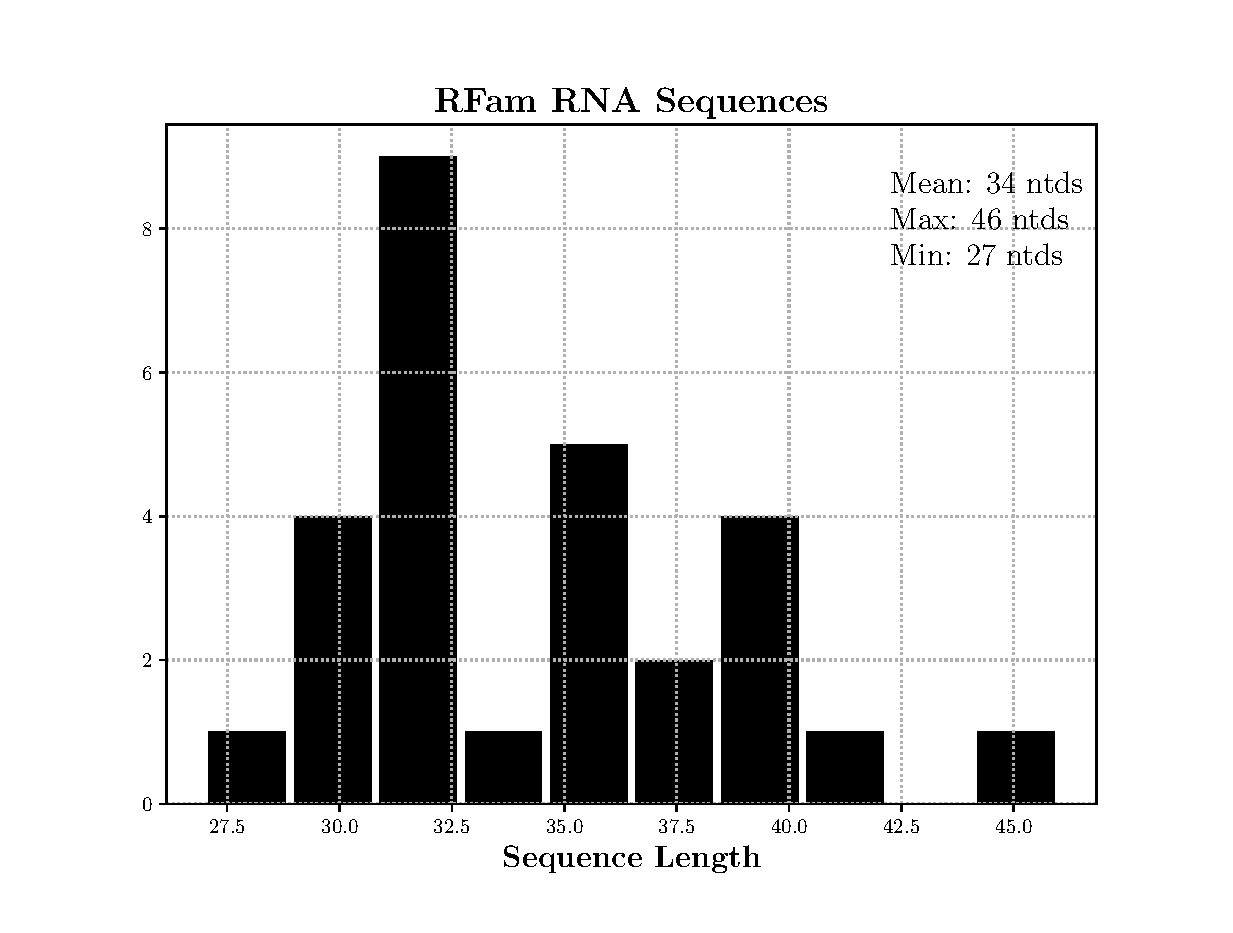
\includegraphics[width = 0.6\textwidth]{fig/rfam}
\caption{The Rfam dataset contains 27 total sequences with variable length. The average length is 34 ntds. The longest sequences is 46 ntds and the shortest sequence is 27 ntds.}
\label{fig:rfam}
\end{figure}
\end{multicols}

\begin{multicols}{2}
\section{CNN Predicts Secondary Structure}
Convolutional neural networks (CNN)s are machine learning algorithms that are primarily used for image classification problems. The input layer is the image’s RGB values, which are then fed through multiple convolution layers, that are finally connected to a standard fully-connected feed forward neural network. Ultimately, to use a CNN one must have data that can be interrupted as an image. Following \cite{10.3389/fgene.2019.00467}, we have replicated their CNN in PyTorch \cite{paszke2017automatic} in efforts to achieve similar results.


\subsection{Matrix Representation of RNA}

RNA sequences are comprised of any combination of four nucleotide bases: adenine (A), guanine (G), cytosine (C), and uracil (U). When using ML techniques for RNA secondary structure prediction, a formidable challenge is how to encode the sequence as input for the ML architecture. We have chosen to encode the sequence as a matrix in order to use a CNN architecture. The rules of folding a RNA secondary structure are very simple: A pairs with U, G pairs with C, and sometimes G pairs with C. The canonical pairs A-U and G-C are called Watson-Crick pairs (CITE), while the G-U pair is known as the wobble pair. Following these simple rules, we can build a weighted matrix based on which base is more likely to pair with whom. The complete matrix building algorithm is explain in \cite{10.3389/fgene.2019.00467}, and our source code is available on this \href{https://github.com/harrisonlabollita/RNA-ML/blob/master/src/explore/cnn%20code/rna2matrix.py}{GitHub repository}.

\subsection{Model}

The architecture of our CNN is simple. The  model contains two convolutional layers, two pooling layers, and three fully-connected layers. We use a binary cross-entropy loss function, since we are predicting either a value of 0 or 1. We optimized the hyperparameters in our model via configuration space searching, where we randomly choose parameters from our configuration space, train our network and log the performance. We found that a learning rate of 0.001 and momentum of 0.9 performed the best without overfitting.

We have illustrated the workflow of our CNN Model in Figure \ref{fig:cnn_model}. We begin with an RNA sequence, convert the sequence into a matrix, then feed it into our CNN. The output of the CNN is a $N \times 3$ matrix, where $N$ is the number of nucleotides in the sequence and our model's predicted values of each nucleotide being paired or unpaired. From this information, we reconstuct the dotbracket representation by choosing the highest value in each row as the model's choice for paired ("(" or ")") or unpaired (".") and compare our predicted structure with the actual secondary structure for this sequence.
\end{multicols}

\begin{figure}[H]
\centering
\hspace*{-8cm}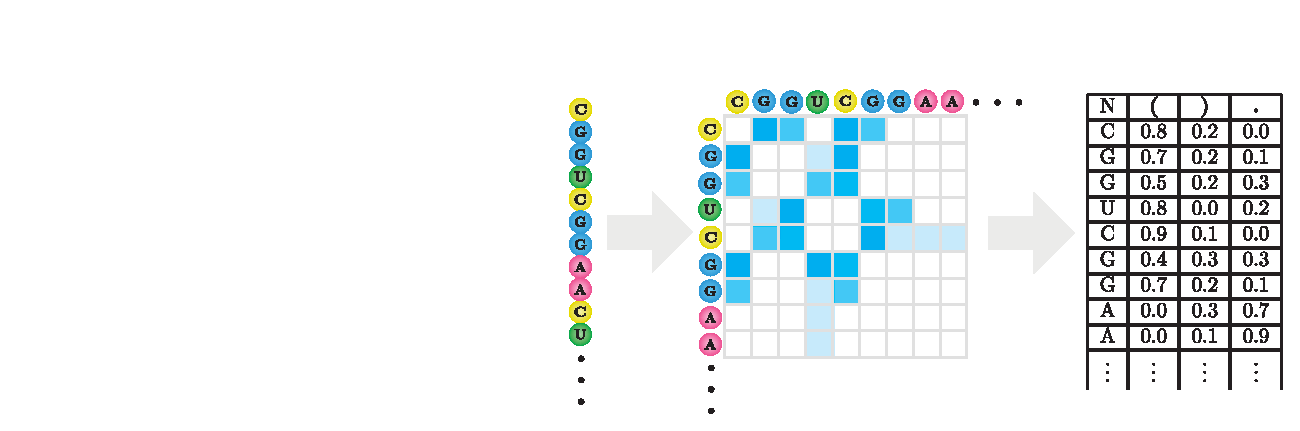
\includegraphics{fig/cnn_model_outline}
\caption{We convert our dataset of RNA sequences into a new dataset of RNA matrices. These matrices are used as inputs into our CNN. Notice that the darker blue squares correspond to heavier weighted base meaning more likely to be paired. The output of our network is the matrix on the far right which we use to reconstruct the dot bracket represenation of the secondary structure.}
\label{fig:cnn_model}
\end{figure}

\begin{multicols}{2}
We trained and validated our CNN model on dataset containing 50,000 uniform length RNA sequences following the standard condition, where 80\% of the data is used for training and 20\% of the dataset was used for validation. We trained our network for 100 epochs with a batchsize of 100. We quantified the accuracy of our model by counting the number of mistakes our model made when predicting the secondary structure. A perfect prediction corresponds to 0 mistakes.
\end{multicols}

\begin{multicols}{2}
\subsection{Results and Discussion}
In this section, we present our CNN model's performance on RNA secondary structure prediction. In Figure \ref{fig:acc}, we have plotted the training and validation accuracy of our model throughout the training session. We can see that the model converges to about 84\% accuracy for both training and validation accuracies.

Our CNN model achieves similar results to the \cite{10.3389/fgene.2019.00467}, however, our model will sometimes predict non-physical structures. Therefore, it is necessary that we include a dynamic layer in our model that corrects for these non-physical outputs. This is the central weakness of all non-physical secondary structure predictors. Without including knowledge of physical considerations these models will always produce unphysical secondary structures.

\end{multicols}
\begin{figure}[H]
\centering
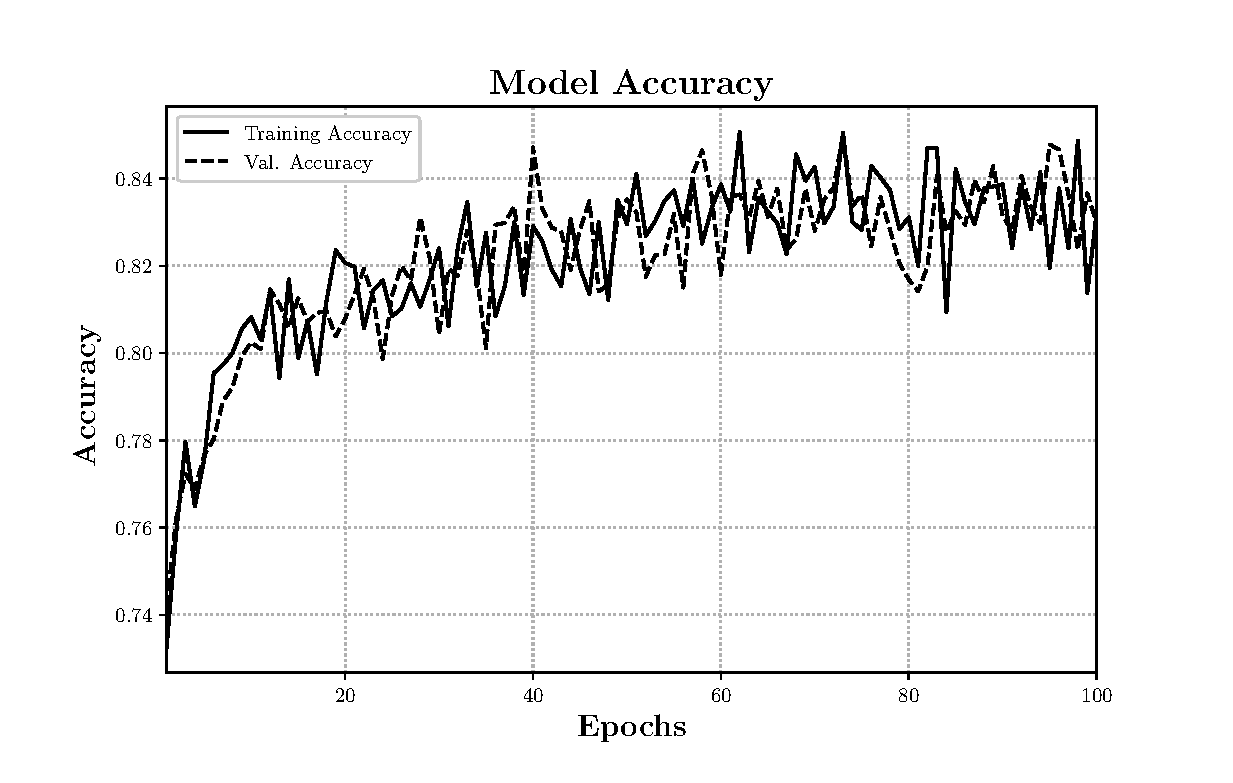
\includegraphics[width = \textwidth]{fig/acc}
\caption{Training and validation accuracy over the 100 epochs. The solid black line is the training accuracy and the dotted black line is the validation accuracy.}
\label{fig:acc}
\end{figure}



\section{Stem Level Gillespie Algorithm}
\subsection{Introduction to Gillespie Algorithm}
In \cite{10.1093/nar/gkv480}, the following alogrithm is presented:
\begin{enumerate}
\item Extract the total flux $\Phi$ from the partial sum table.
\item Choose two random numbers $r_{1}$ and $r_{2}$ on the interval $[0, 1]$.
\item  Increment the time by $\tau = - \ln(r_{2})/\Phi$.
\item Identify the first *stem* which satisfies the inequality $$ \sum_{\ell =1} \phi_{\ell} \geq r_{1} \Phi$$ by using our table of reaction rates for each stem. We then recalculate the remainder $\Phi = r_{1} \Phi - \sum_{\ell = 1} \phi_{\ell}$ on the fly.
\item Once this condition is met we choose this stem to form. We make sure it is compatible with all of the other stems in the current structure. If it is not compatible with the current structure, we remove the incompatible pieces and add our new stem. However, if adding this move requires breaking almost all of the current stems then we do not allow this move to occur.
\item Go to Step 1 until the the arbitraty cutoff time has been reached.
\end{enumerate}

\subsection{Stem Level Implementation}

\begin{figure}[H]
\centering
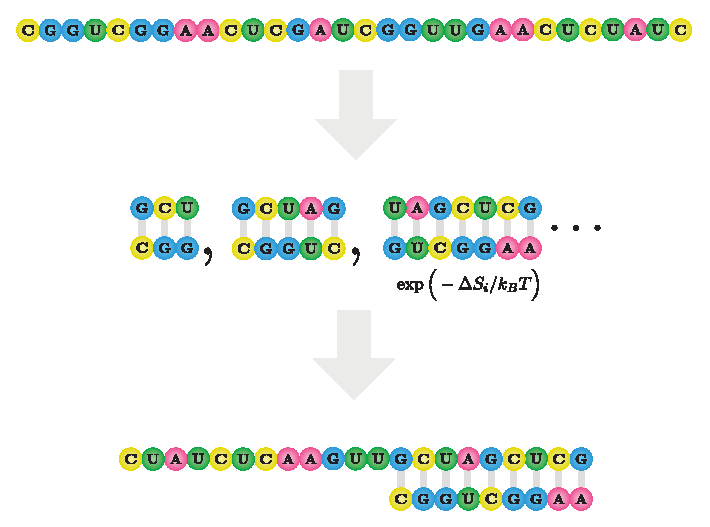
\includegraphics{fig/rna_gillespie_algo}
\end{figure}

\subsection{Results}

\begin{multicols}{2}
\begin{figure}[H]
\centering
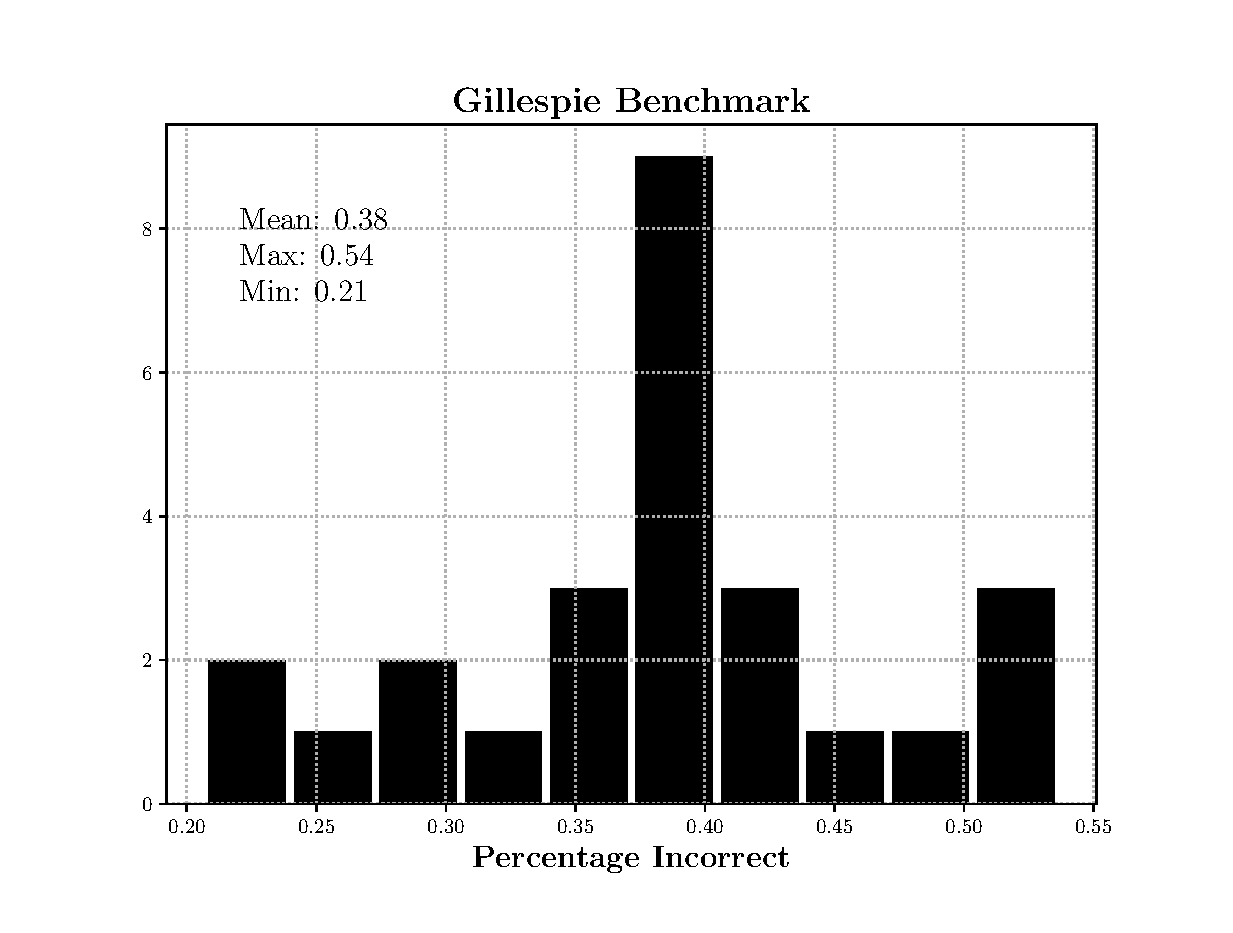
\includegraphics[width = 0.55\textwidth]{fig/gill_bench}
\caption{}
\label{fig:gill}
\end{figure}
\begin{figure}[H]
\centering
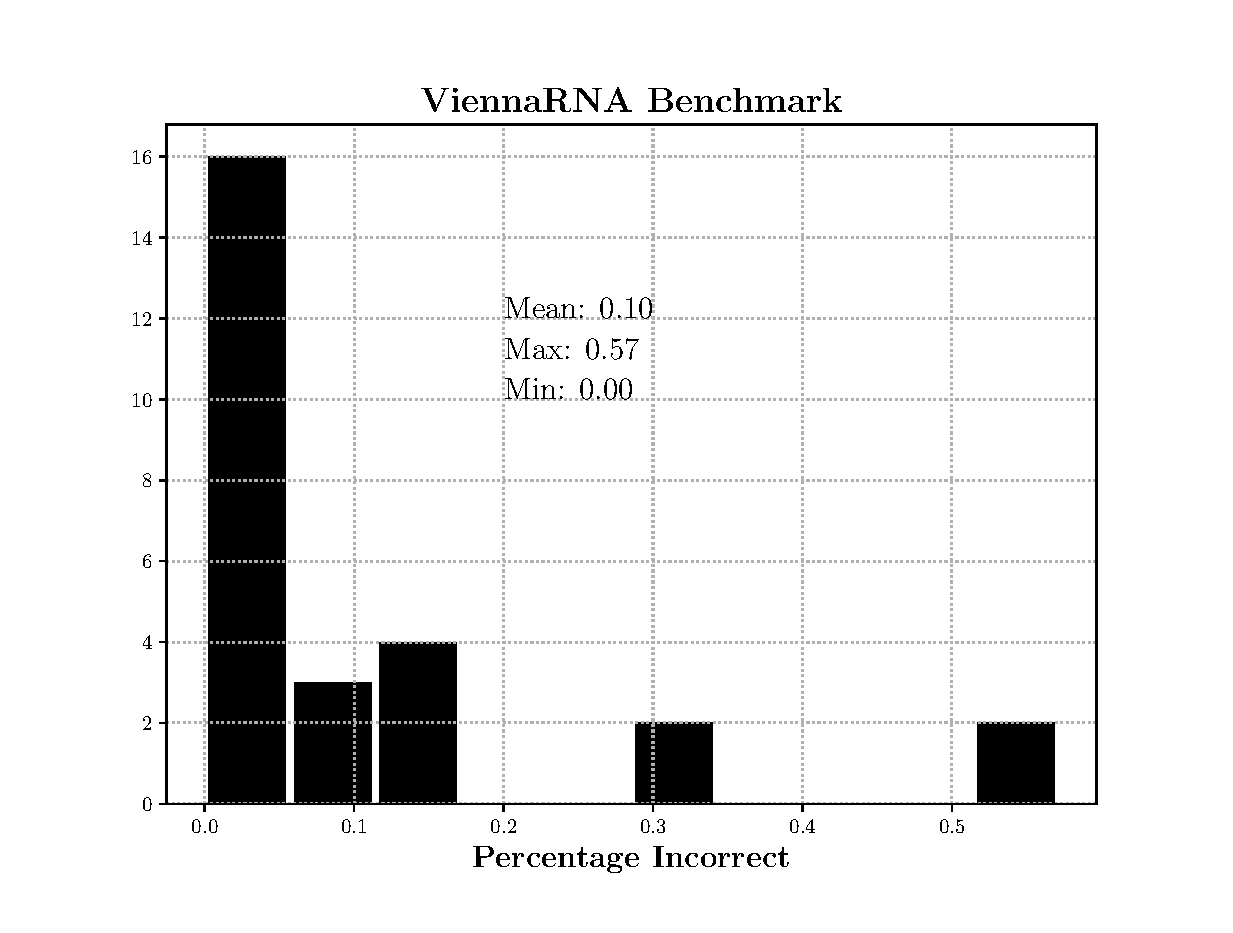
\includegraphics[width = 0.55\textwidth]{fig/v_rna_bench}
\caption{}
\label{fig:vbench}
\end{figure}
\end{multicols}
\section{Conclusion}

\newpage
\nocite{*}
\printbibliography
\end{document}
